% !Mode:: "TeX:UTF-8"
% !TeX program = xelatex
\documentclass[bachelor,ktreport,openany,oneside,AutoFakeBold=true]{buaathesis}

\usepackage{float}
\usepackage{tikz}
\usepackage{upquote}

\usetikzlibrary{arrows.meta,positioning,shapes.geometric}

\setmonofont{Consolas}
\graphicspath{{figures/experiment2/}{figures/}{figure/}}
\setlength{\headheight}{16pt}
\hypersetup{
  hidelinks,
  pdftitle={实验二：IIR 数字滤波器设计及软件实现},
  pdfauthor={傅粱训},
  pdfsubject={数字信号处理实验报告}
}

\newcommand{\Hz}{\mathrm{Hz}}
\newcommand{\dd}{\mathrm{d}}

\begin{document}

\degree{数字信号处理实验}{Course}{数字信号处理实验}{数字信号处理实验}
\ktclass{数字信号处理实验报告}
\school{未来空天技术}{School of Future Aerospace Technology}
\major{工科试验班（未来空天领军计划）}{Engineering Experimental Class}
\class{242311班}
\thesistitle{实验二：IIR 数字滤波器设计}{及软件实现}{Experiment 2: IIR Digital Filter Design}{and Software Implementation}
\studentID{24373088}
\thesisauthor{傅粱训}{Fu Liangxun}
\teacher{白桐老师}{Bai Tong}
\thesisdate{2026}{6}

\ckeyword{IIR 数字滤波器；椭圆滤波器；抑制载波调幅；频域分离；FFT}
\ekeyword{IIR filter; elliptic filter; SCAM; frequency separation; FFT}

\pagestyle{mainmatter}
\maketitle

\pagestyle{frontmatter}
\begin{cabstract}
本实验围绕 IIR 数字滤波器设计与软件实现展开。实验首先产生三路抑制载波单频调幅信号，并将其相加得到复合信号。三路信号在时域叠加后难以直接分辨，但其频率分量分别位于 \(225\,\Hz\)、\(275\,\Hz\)、\(450\,\Hz\)、\(550\,\Hz\)、\(900\,\Hz\) 和 \(1100\,\Hz\)，在频域中互不重叠，因此可以通过低通、带通和高通滤波器进行分离。

程序使用 Python 信号处理函数设计三个椭圆 IIR 数字滤波器，通带最大衰减取 \(R_p=0.1\,\mathrm{dB}\)，阻带最小衰减取 \(R_s=60\,\mathrm{dB}\)。实验结果显示，低通、带通和高通滤波器阶数分别为 7、6、9，均满足通阻带指标。滤波输出的频谱表明，三个滤波器能够分别保留目标频段并抑制其他信号成分，从而实现复合调幅信号的频域分离。
\end{cabstract}

\begin{eabstract}
This experiment focuses on the design and software implementation of IIR digital filters. Three suppressed-carrier amplitude-modulated signals are generated and summed into a composite signal. Although the components are mixed in the time domain, their spectral lines are separated in the frequency domain, which makes filter-based separation feasible.

Three elliptic IIR filters are designed in Python, including a low-pass filter, a band-pass filter, and a high-pass filter. The maximum passband loss is \(0.1\,\mathrm{dB}\), and the minimum stopband attenuation is \(60\,\mathrm{dB}\). The obtained filter orders are 7, 6, and 9, respectively. The filtering results show that the desired spectral components are preserved while the other components are suppressed, verifying the effectiveness of frequency-domain separation using IIR filters.
\end{eabstract}

\tableofcontents
\cleardoublepage
\phantomsection
\addcontentsline{toc}{chapter}{图目录}
\listoffigures
\cleardoublepage
\phantomsection
\addcontentsline{toc}{chapter}{表目录}
\listoftables

\mainmatter
\pagestyle{mainmatter}

\chapter{实验目的}

本实验围绕 IIR 数字滤波器设计与软件实现展开。通过调用 Python 信号处理函数设计低通、带通和高通三个椭圆数字滤波器，将由三路抑制载波调幅信号相加得到的复合信号分离出来。实验中需要观察复合信号和滤波输出的时域波形及频谱，理解频域分离的基本思想，并掌握根据通带、阻带指标设计 IIR 数字滤波器的方法。

\chapter{实验原理}

\section{抑制载波调幅信号的频谱}

一路抑制载波单频调幅信号可写为
\begin{equation}
s(t)=\cos(2\pi f_m t)\cos(2\pi f_c t),
\end{equation}
其中，\(f_c\) 为载波频率，\(f_m\) 为调制信号频率。利用积化和差公式可得
\begin{equation}
s(t)=\frac{1}{2}\cos\left[2\pi(f_c-f_m)t\right]
    +\frac{1}{2}\cos\left[2\pi(f_c+f_m)t\right].
\end{equation}
因此一路抑制载波调幅信号只有两个频率分量，分别位于 \(f_c-f_m\) 和 \(f_c+f_m\)，并且关于载波频率 \(f_c\) 对称。三路信号在时域相加后互相混叠，但只要频谱互不重叠，就可以通过滤波器在频域将其分离。

本实验采样频率和采样点数为
\begin{equation}
F_s=10000\,\Hz,\qquad N=1600.
\end{equation}
三路信号参数如表 \ref{tab:signal-param} 所示。

\begin{table}[H]
\centering
\caption{三路抑制载波调幅信号参数}
\label{tab:signal-param}
\begin{tabular}{ccccc}
\toprule
信号 & 载波频率 \(f_c/\Hz\) & 调制频率 \(f_m/\Hz\) & 差频/\(\Hz\) & 和频/\(\Hz\)\\
\midrule
\(x_1(t)\) & 1000 & 100 & 900 & 1100\\
\(x_2(t)\) & 500 & 50 & 450 & 550\\
\(x_3(t)\) & 250 & 25 & 225 & 275\\
\bottomrule
\end{tabular}
\end{table}

\section{椭圆 IIR 数字滤波器}

IIR 数字滤波器的一般系统函数为
\begin{equation}
H(z)=\frac{B(z)}{A(z)}
=\frac{b_0+b_1z^{-1}+\cdots+b_Mz^{-M}}
{1+a_1z^{-1}+\cdots+a_Nz^{-N}}.
\end{equation}
椭圆滤波器在通带和阻带均具有等波纹特性，在相同通阻带指标下通常能以较低阶数满足设计要求。本实验要求通带最大衰减为 \(R_p=0.1\,\mathrm{dB}\)，阻带最小衰减为 \(R_s=60\,\mathrm{dB}\)。若定义滤波器损耗函数为
\begin{equation}
A(f)=-20\log_{10}\left|H\left(e^{j2\pi f/F_s}\right)\right|,
\end{equation}
则通带和阻带指标分别表示为
\begin{equation}
A(f)\le R_p,\quad f\in \Omega_p,
\qquad
A(f)\ge R_s,\quad f\in \Omega_s.
\end{equation}

根据复合信号的频谱位置，三个滤波器的通带和阻带频率选取如表 \ref{tab:filter-param} 所示。程序中使用 \texttt{scipy.signal.ellipord} 求满足指标的最低阶数，再使用 \texttt{scipy.signal.ellip} 得到二阶节形式的 IIR 滤波器，并用 \texttt{sosfilt} 进行滤波实现。

\begin{table}[H]
\centering
\caption{三个椭圆滤波器的设计指标}
\label{tab:filter-param}
\begin{tabular}{ccccc}
\toprule
滤波器 & 分离信号 & 通带频率/\(\Hz\) & 阻带频率/\(\Hz\) & 阶数\\
\midrule
低通 & \(y_3(n)\) & \(0\sim 300\) & \(400\sim 5000\) & 7\\
带通 & \(y_2(n)\) & \(400\sim 600\) & \(0\sim 350,\ 700\sim 5000\) & 6\\
高通 & \(y_1(n)\) & \(800\sim 5000\) & \(0\sim 700\) & 9\\
\bottomrule
\end{tabular}
\end{table}

\chapter{实验内容与结果分析}

\section{主程序框图}

实验主程序流程如图 \ref{fig:flowchart2} 所示。程序先产生三路抑制载波调幅信号并相加得到 \(s(t)\)，然后根据频谱分布分别设计低通、带通和高通椭圆滤波器，最后对复合信号滤波并绘制输出信号的时域和频域结果。

\begin{figure}[H]
\centering
\begin{tikzpicture}[
  node distance=8mm,
  process/.style={rectangle, draw, rounded corners=2pt, align=center, minimum width=9.8cm, minimum height=9mm},
  startstop/.style={ellipse, draw, align=center, minimum width=3.0cm, minimum height=8mm},
  arrow/.style={-{Stealth[length=2.2mm]}, thick}
]
\node[startstop] (start) {开始};
\node[process, below=of start] (signal) {设置 \(F_s=10000\,\Hz,\ N=1600\)，产生三路 SCAM 信号并相加得到 \(s(t)\)};
\node[process, below=of signal] (spectrum) {绘制 \(s(t)\) 的时域波形和 \(N\) 点 FFT 幅频特性};
\node[process, below=of spectrum] (filters) {按 \(R_p=0.1\,\mathrm{dB}, R_s=60\,\mathrm{dB}\) 设计低通、带通、高通椭圆滤波器};
\node[process, below=of filters] (loss) {计算并绘制三个滤波器的损耗函数曲线};
\node[process, below=of loss] (filtering) {用三个滤波器对 \(s(t)\) 滤波，得到 \(y_1(n),y_2(n),y_3(n)\)};
\node[process, below=of filtering] (output) {绘制三路输出的时域波形和幅频特性，分析分离效果};
\node[startstop, below=of output] (end) {结束};

\draw[arrow] (start) -- (signal);
\draw[arrow] (signal) -- (spectrum);
\draw[arrow] (spectrum) -- (filters);
\draw[arrow] (filters) -- (loss);
\draw[arrow] (loss) -- (filtering);
\draw[arrow] (filtering) -- (output);
\draw[arrow] (output) -- (end);
\end{tikzpicture}
\caption{实验二主程序框图}
\label{fig:flowchart2}
\end{figure}

\section{复合信号的时域波形与频谱}

由三路信号相加得到的复合信号为
\begin{equation}
s(t)=x_1(t)+x_2(t)+x_3(t).
\end{equation}
其时域波形和单边幅频特性如图 \ref{fig:mixed} 所示。可以看到，时域波形中三路调幅信号已经叠加在一起，不能直接分辨；但频谱上出现 \(225\,\Hz\)、\(275\,\Hz\)、\(450\,\Hz\)、\(550\,\Hz\)、\(900\,\Hz\)、\(1100\,\Hz\) 六根谱线，三路信号在频域是分开的，因此可以用滤波器进行分离。

\begin{figure}[H]
\centering
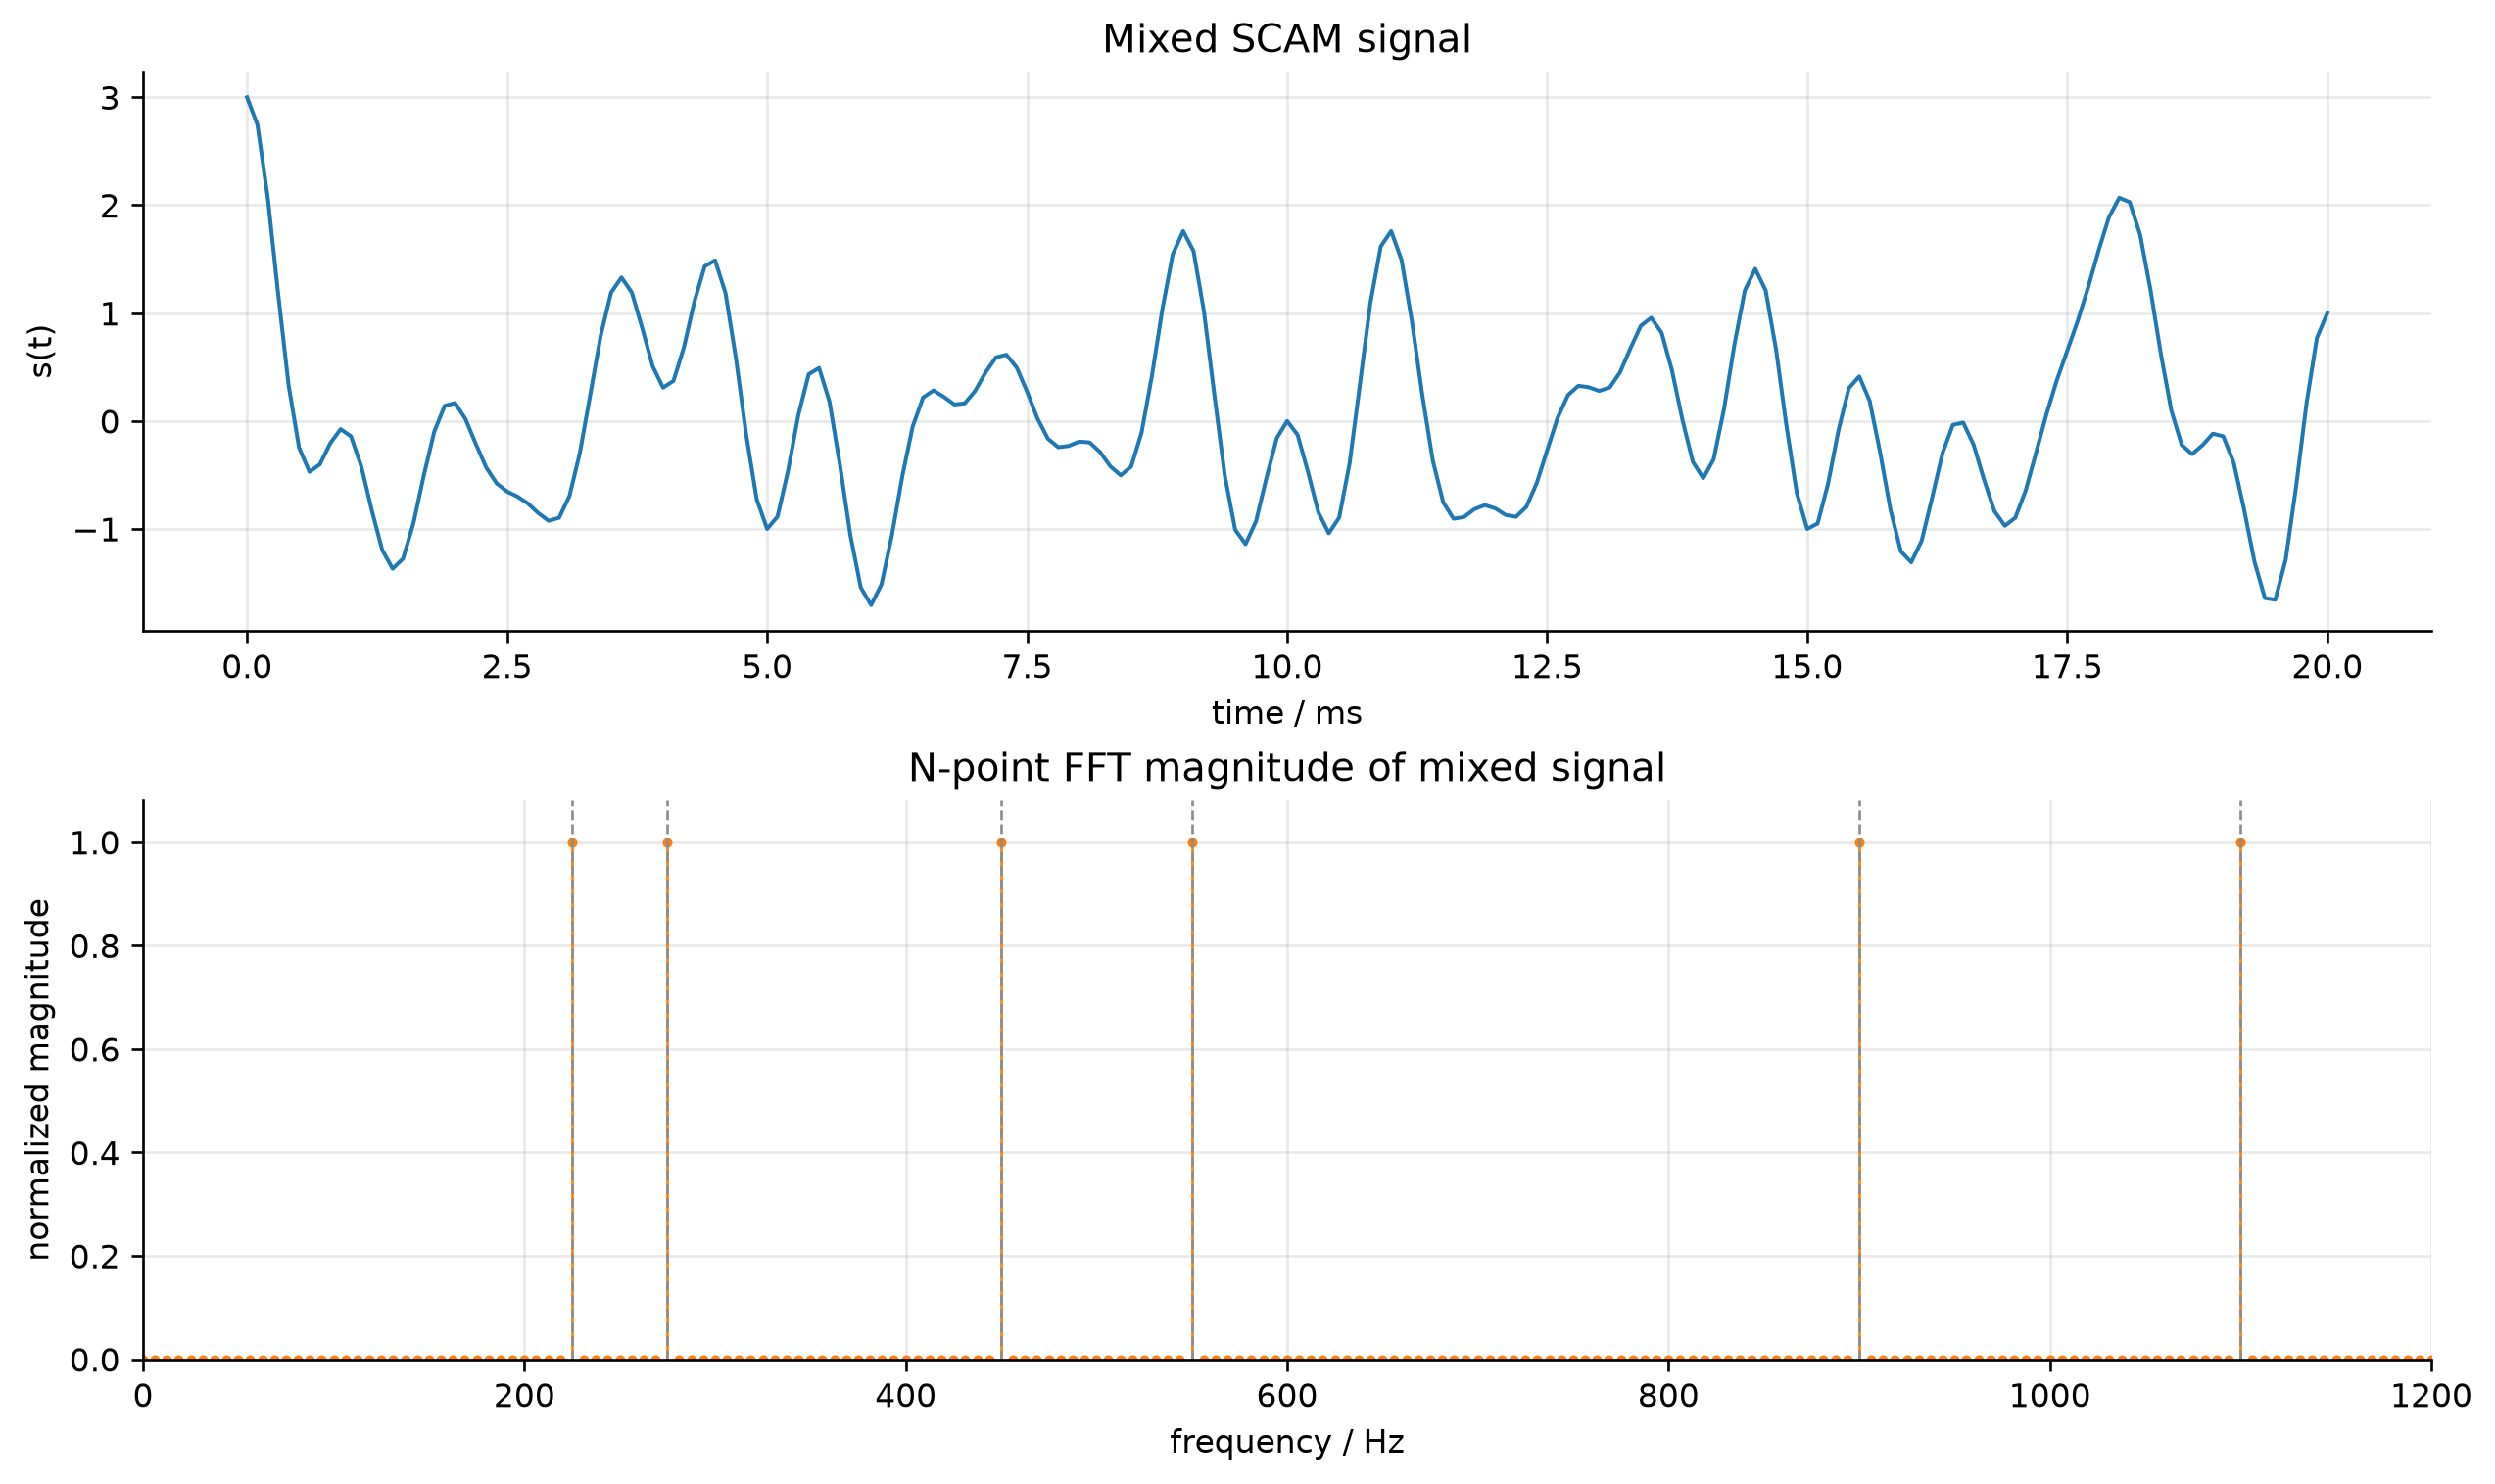
\includegraphics[width=0.95\textwidth]{mixed_signal.png}
\caption{复合信号 \(s(t)\) 的时域波形和幅频特性}
\label{fig:mixed}
\end{figure}

\section{滤波器损耗函数}

三个滤波器的损耗函数如图 \ref{fig:loss} 所示。程序计算得到低通、带通、高通滤波器的阶数分别为 7、6、9；在各自通带内最大损耗均为 \(0.1000\,\mathrm{dB}\)，在阻带内最小衰减均达到 \(60.0000\,\mathrm{dB}\)。这说明所设计的椭圆滤波器满足题目要求。

\begin{figure}[H]
\centering
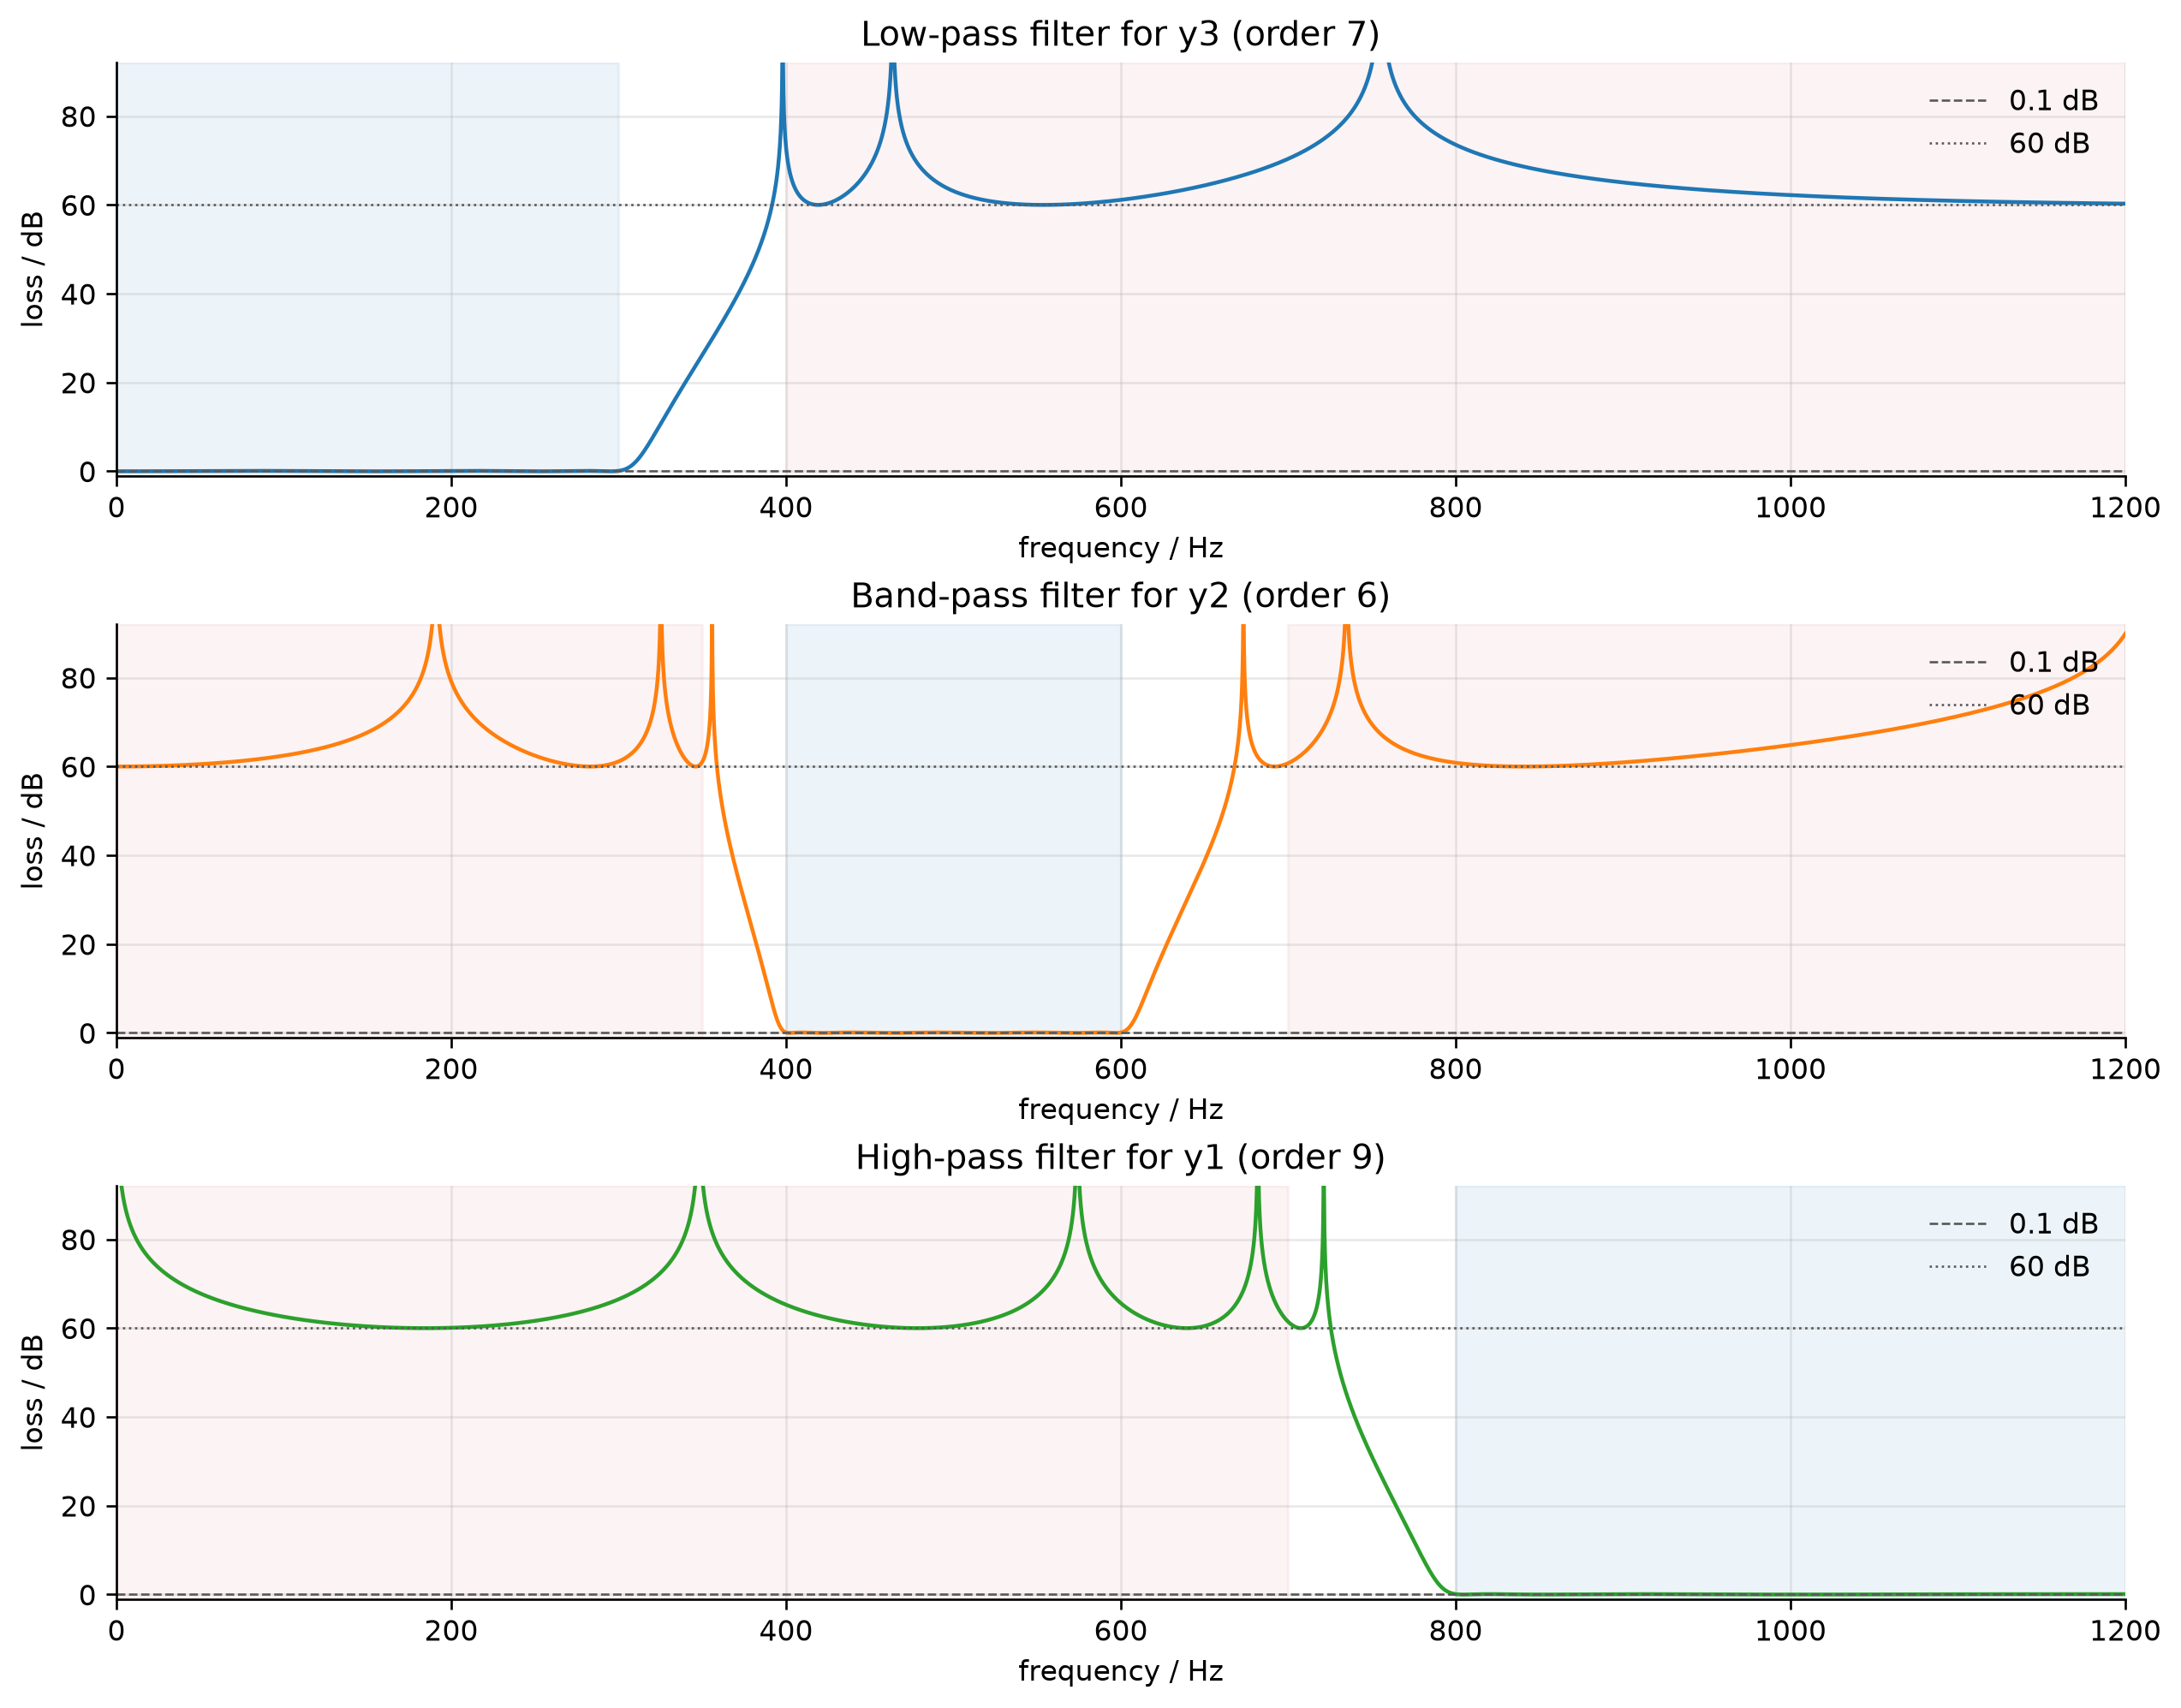
\includegraphics[width=0.95\textwidth]{filters_loss.png}
\caption{三个椭圆分离滤波器的损耗函数曲线}
\label{fig:loss}
\end{figure}

\section{滤波分离结果}

使用三个滤波器分别对复合信号 \(s(t)\) 进行滤波，分离结果如图 \ref{fig:separated} 所示。由于 IIR 滤波器在起始阶段存在瞬态响应，图中时域波形取 \(20\,\mathrm{ms}\) 以后的一段进行观察。低通滤波器保留 \(225\,\Hz\) 和 \(275\,\Hz\) 附近的谱线，对应 \(f_c=250\,\Hz\) 的第三路信号；带通滤波器保留 \(450\,\Hz\) 和 \(550\,\Hz\) 附近的谱线，对应 \(f_c=500\,\Hz\) 的第二路信号；高通滤波器保留 \(900\,\Hz\) 和 \(1100\,\Hz\) 附近的谱线，对应 \(f_c=1000\,\Hz\) 的第一路信号。由频谱结果可以看出，三路信号被较好分离。

\begin{figure}[H]
\centering
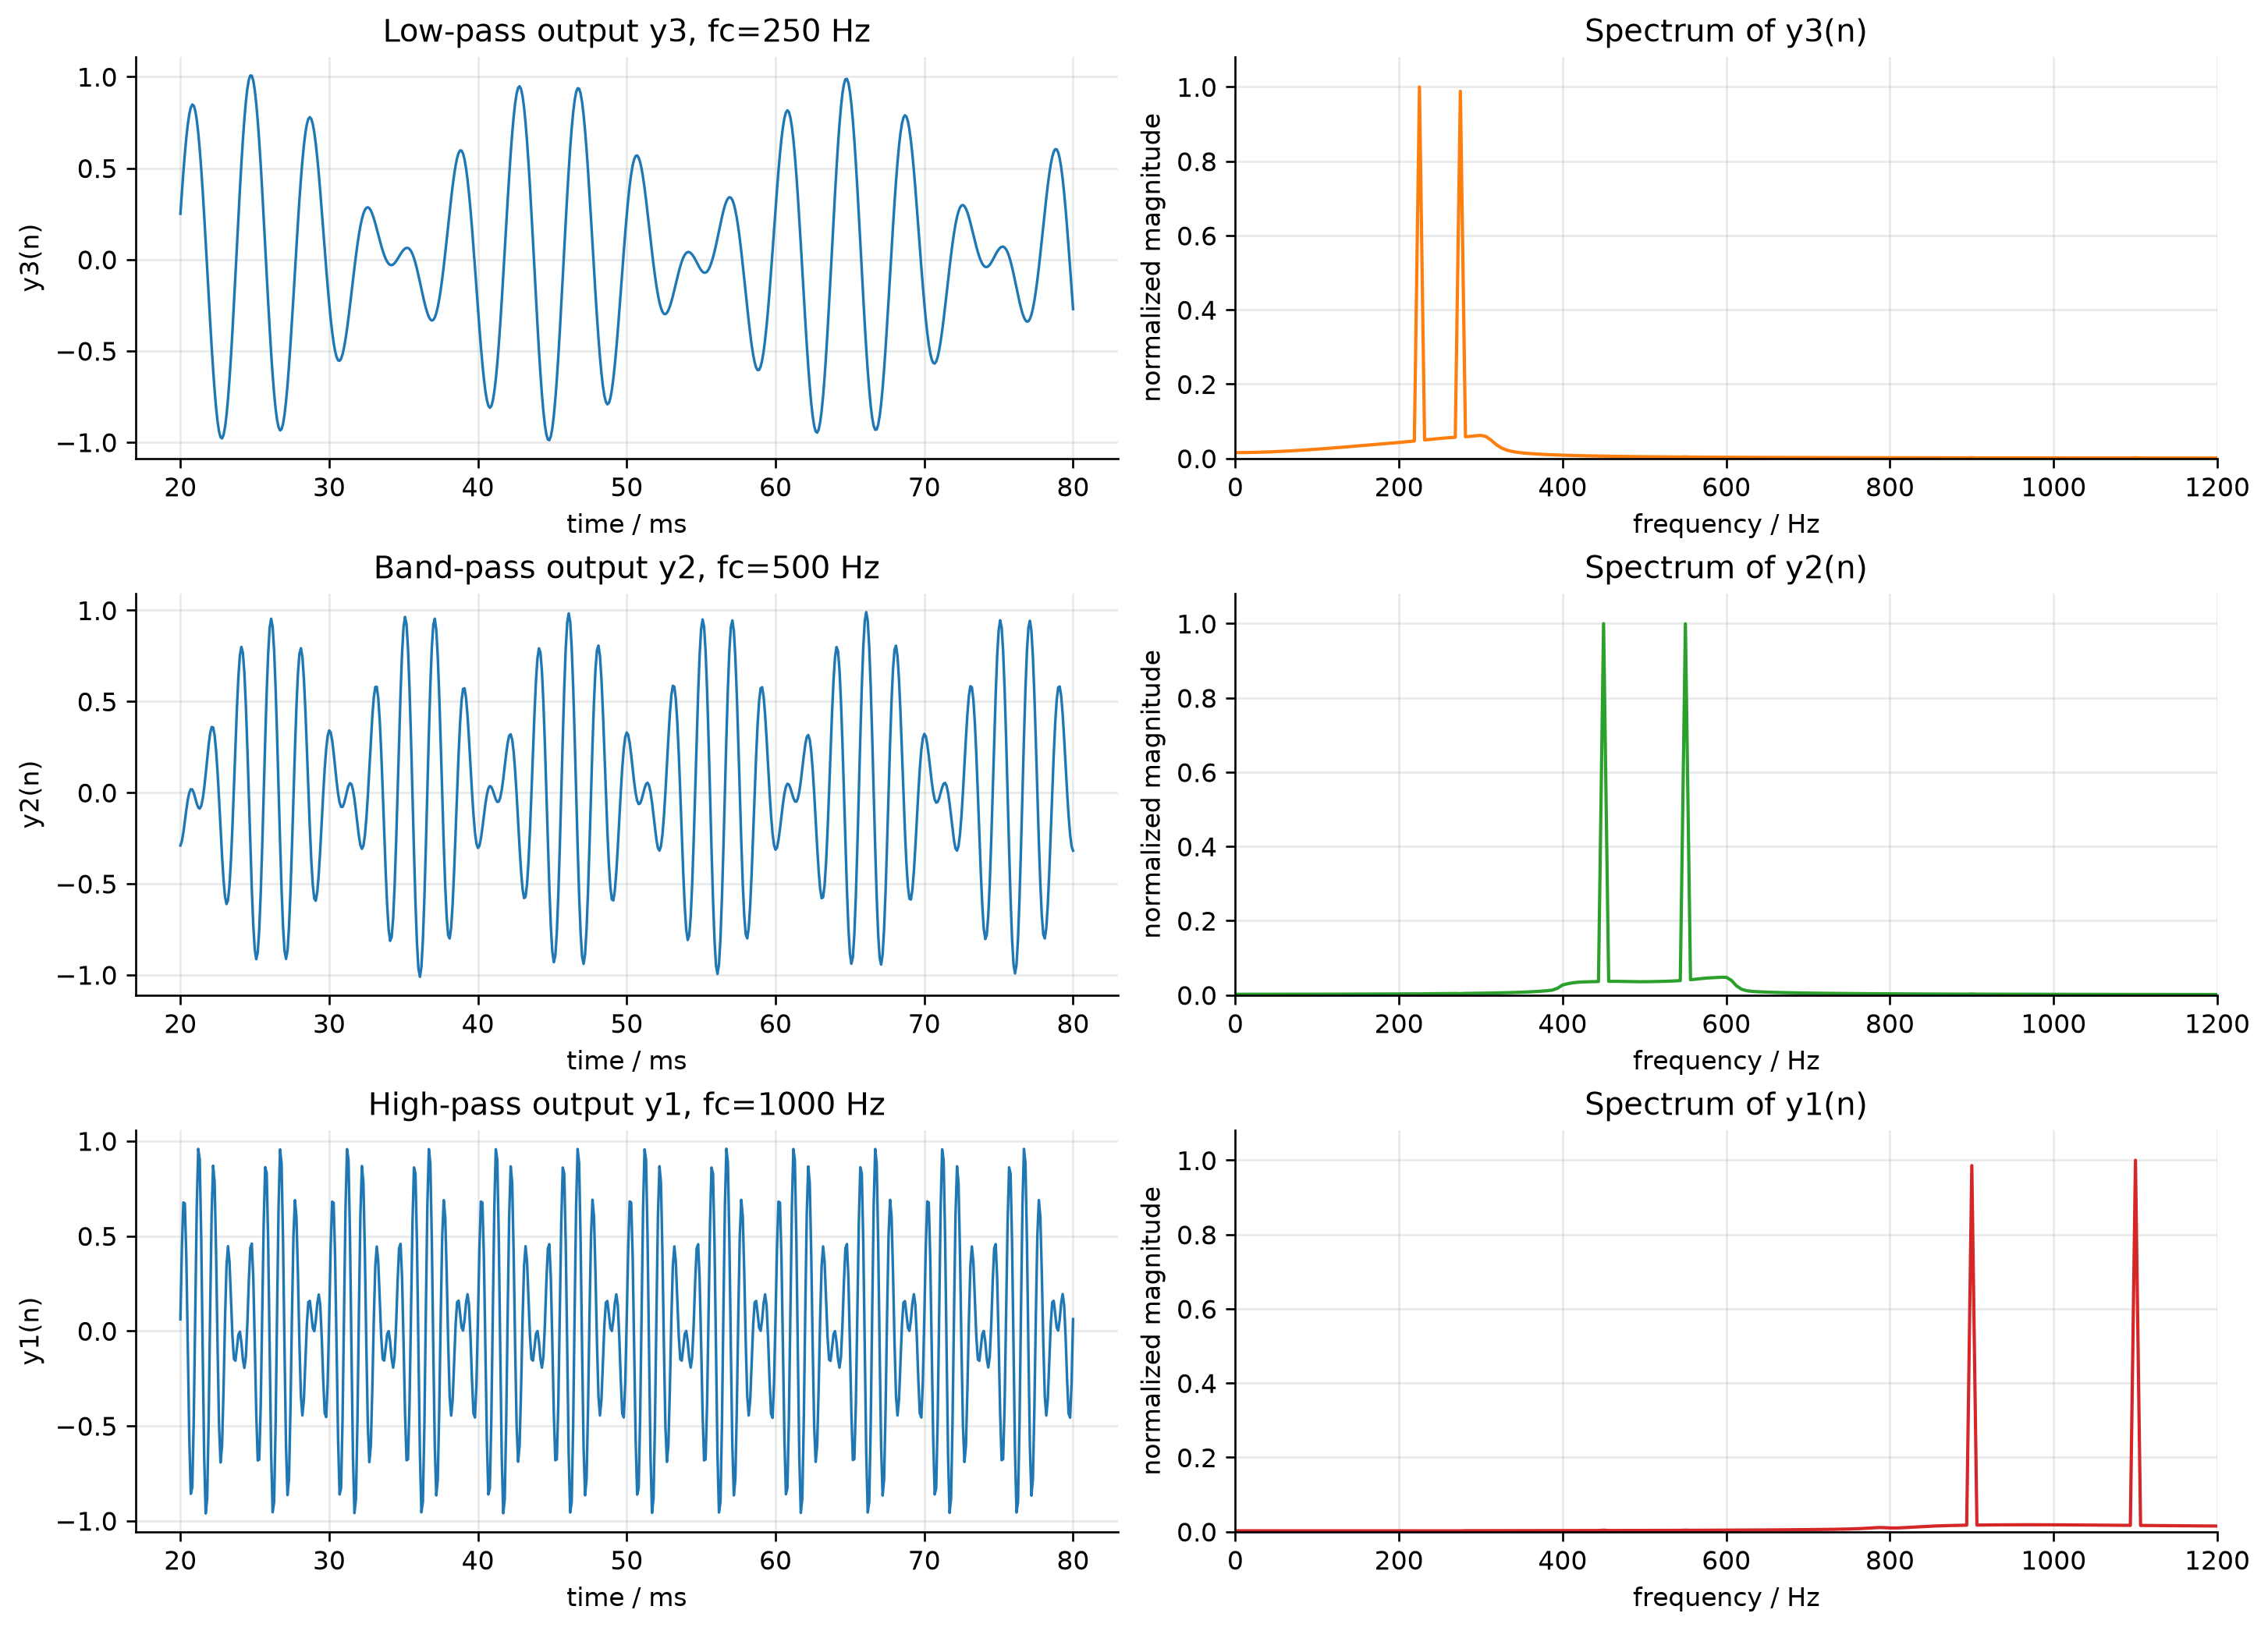
\includegraphics[width=0.98\textwidth]{separated_signals.png}
\caption{三路滤波输出信号的时域波形和幅频特性}
\label{fig:separated}
\end{figure}

\chapter{实验结论}

本实验通过椭圆 IIR 数字滤波器实现了三路抑制载波调幅信号的频域分离。实验结果说明：虽然三路信号在时域相加后难以直接分辨，但其频率成分互不重叠时，可以根据频谱位置设计不同类型的滤波器进行分离。椭圆滤波器在满足 \(0.1\,\mathrm{dB}\) 通带衰减和 \(60\,\mathrm{dB}\) 阻带衰减的条件下阶数较低，适合完成这种过渡带较窄的分离任务。实际软件实现中采用二阶节形式可以提高 IIR 滤波器的数值稳定性。

\chapter{思考题}

\section{确定三路调幅信号的载波频率和调制信号频率}

由信号产生函数可知：
\begin{equation}
f_{c1}=\frac{F_s}{10}=1000\,\Hz,\quad
f_{m1}=\frac{f_{c1}}{10}=100\,\Hz;
\end{equation}
\begin{equation}
f_{c2}=\frac{F_s}{20}=500\,\Hz,\quad
f_{m2}=\frac{f_{c2}}{10}=50\,\Hz;
\end{equation}
\begin{equation}
f_{c3}=\frac{F_s}{40}=250\,\Hz,\quad
f_{m3}=\frac{f_{c3}}{10}=25\,\Hz.
\end{equation}
因此三路抑制载波调幅信号的正频率谱线分别为 \(900\,\Hz\)、\(1100\,\Hz\)，\(450\,\Hz\)、\(550\,\Hz\)，以及 \(225\,\Hz\)、\(275\,\Hz\)。

\section{改变采样点数时是否能得到 6 根理想谱线}

对长度为 \(N\) 的序列作 \(N\) 点 FFT 时，频率分辨率为
\begin{equation}
\Delta f=\frac{F_s}{N}.
\end{equation}
若某一频率 \(f\) 正好落在 DFT 栅格上，则需满足
\begin{equation}
k=\frac{fN}{F_s}
\end{equation}
为整数。否则该频率不能只集中在一个 DFT 频点上，会出现频谱泄漏，因而不能得到理想谱线。

当 \(N=1600\) 时，\(\Delta f=6.25\,\Hz\)，六个频率 \(225,275,450,550,900,1100\,\Hz\) 都落在整数频点上，所以能得到 6 根理想谱线。当 \(N=1800\) 时，\(\Delta f=5.5556\,\Hz\)，其中
\begin{equation}
\frac{225\times 1800}{10000}=40.5,\qquad
\frac{275\times 1800}{10000}=49.5,
\end{equation}
不是整数，因此不能得到全部 6 根理想谱线。虽然 \(450\,\Hz\)、\(550\,\Hz\)、\(900\,\Hz\)、\(1100\,\Hz\) 仍落在整数频点上，但 \(225\,\Hz\) 和 \(275\,\Hz\) 会发生频谱泄漏。当 \(N=2000\) 时，\(\Delta f=5\,\Hz\)，六个频率均为 \(5\,\Hz\) 的整数倍，所以又可以得到 6 根理想谱线。程序验证结果如图 \ref{fig:fft-length} 所示。

\begin{figure}[H]
\centering
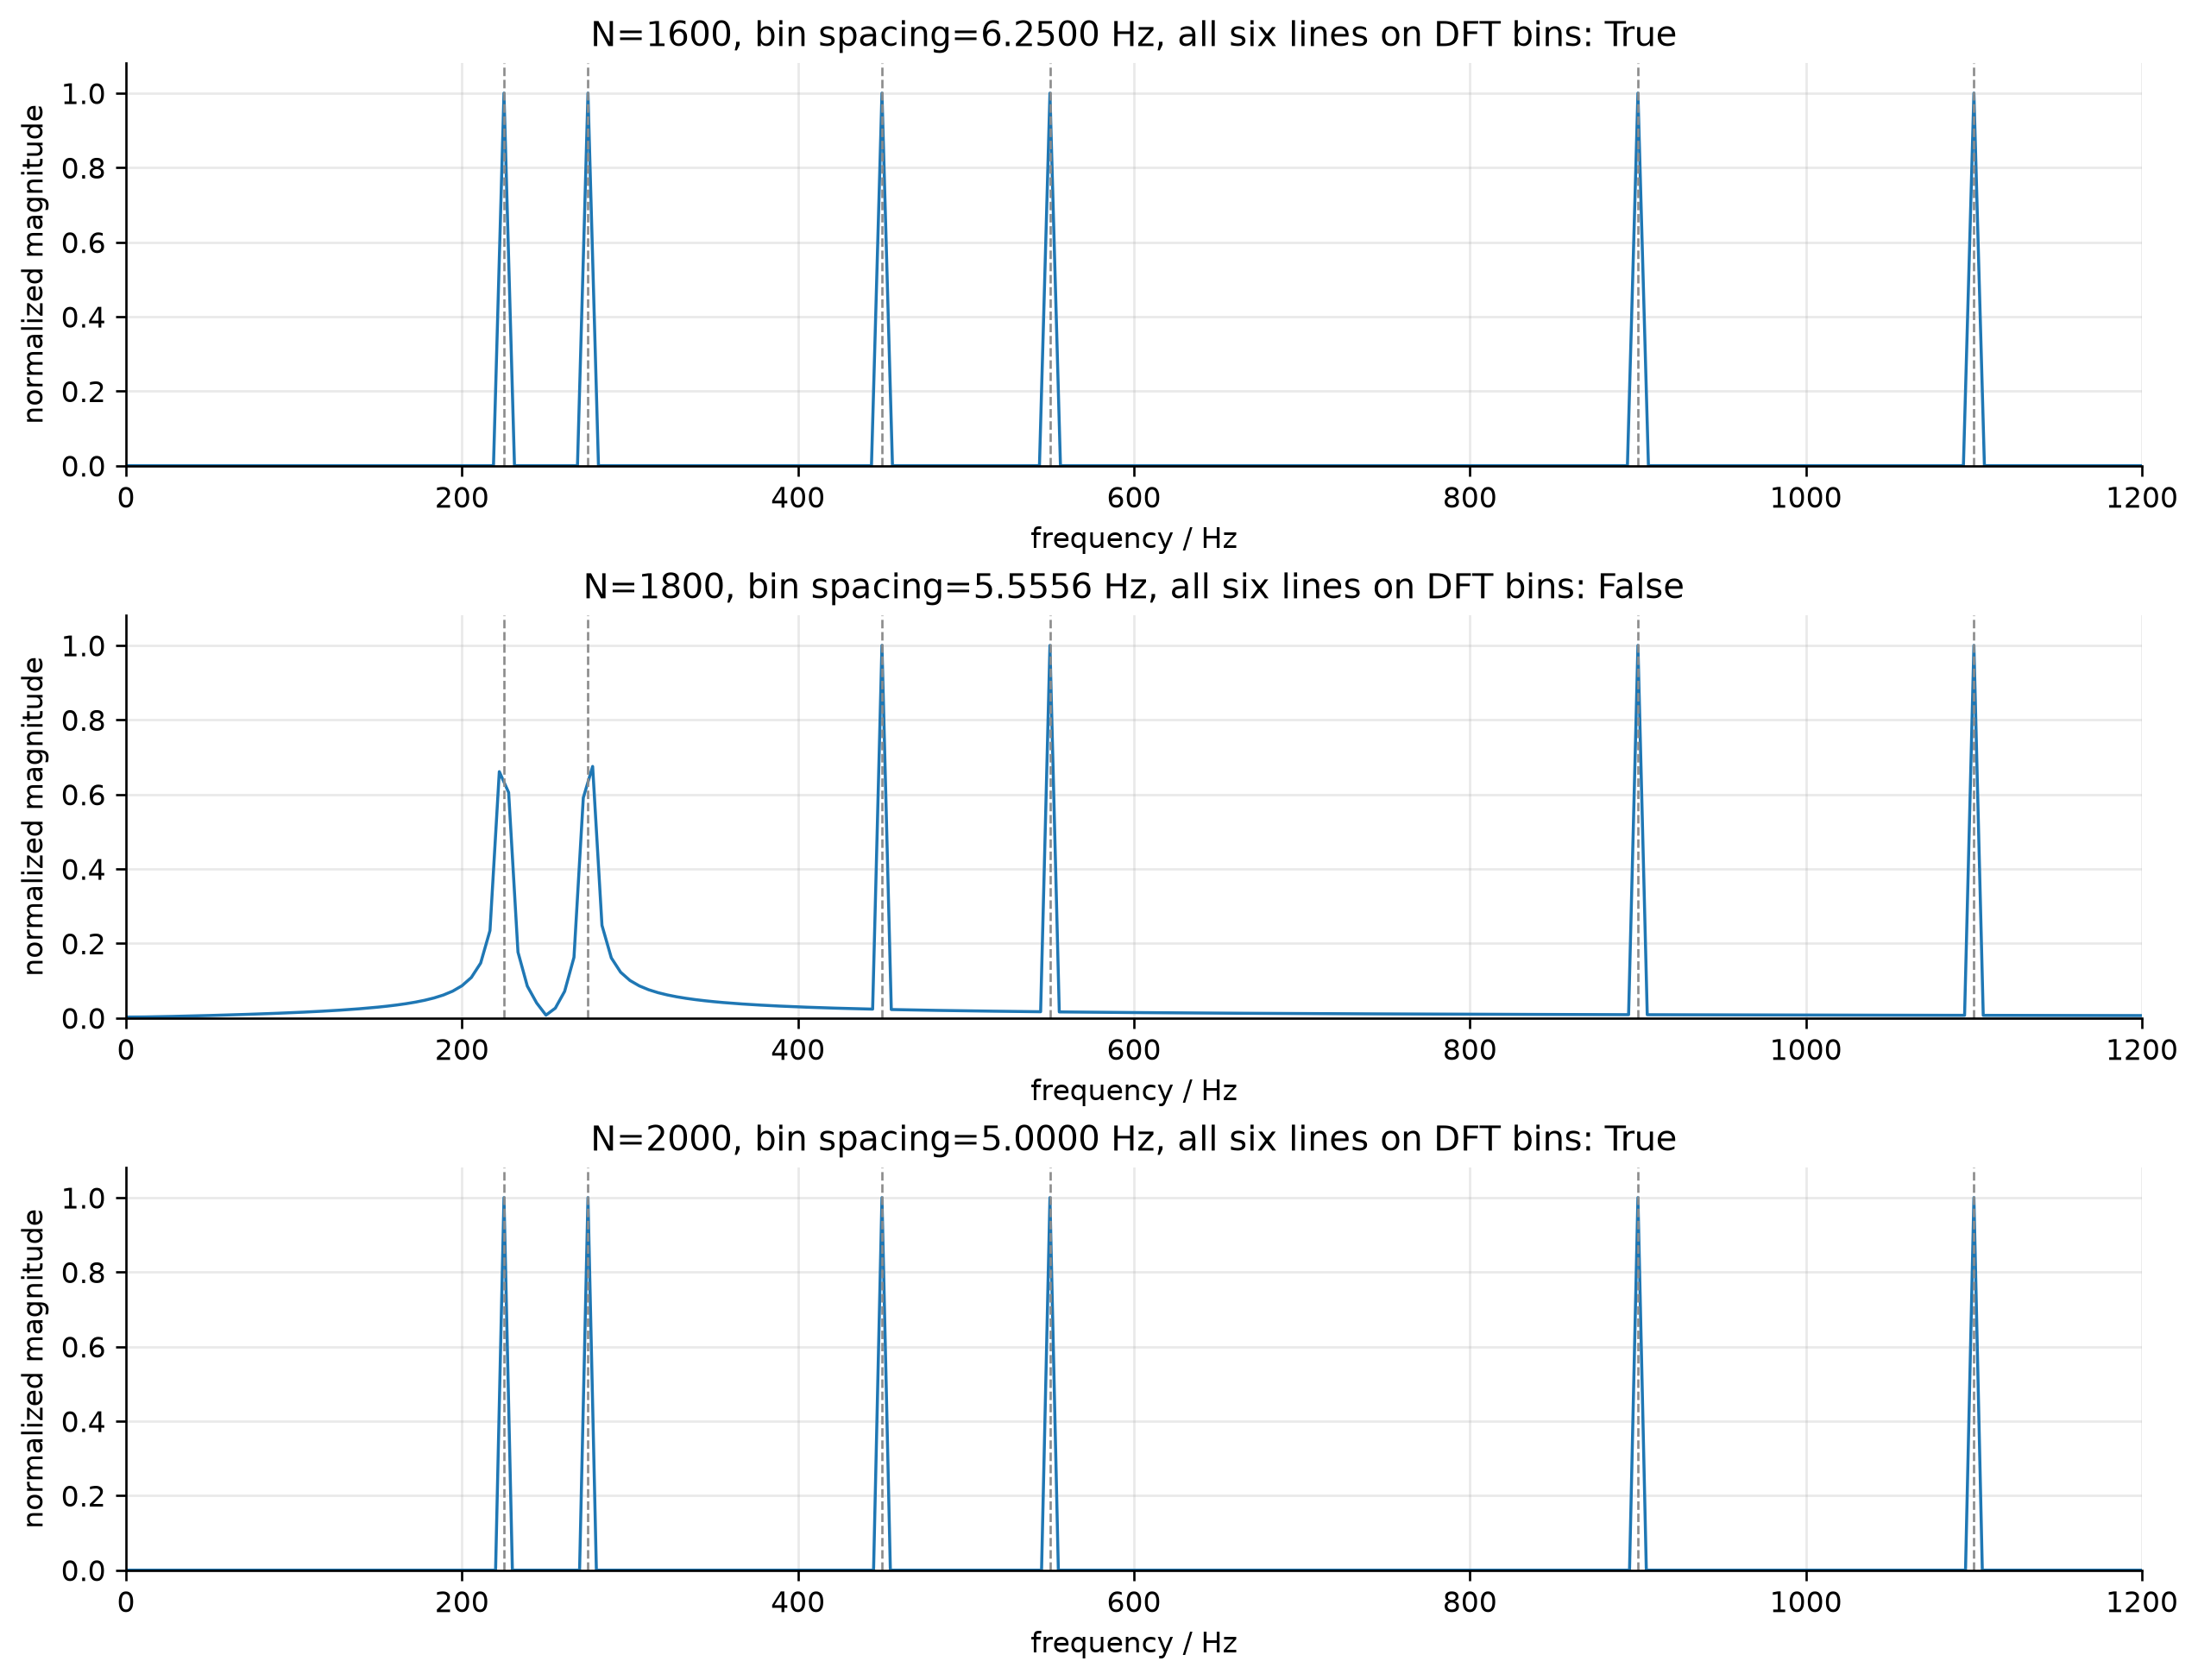
\includegraphics[width=0.95\textwidth]{fft_length_comparison.png}
\caption{不同采样点数下的 FFT 频谱对比}
\label{fig:fft-length}
\end{figure}

\section{加入载波成分后的 AM 信号与 SCAM 信号差别}

将每路信号改为 AM 信号：
\begin{equation}
s_{\mathrm{AM}}(t)=\left[A_0+A_m\cos(2\pi f_m t)\right]\cos(2\pi f_c t),
\end{equation}
本实验取 \(A_0=A_m=1\)。展开可得
\begin{equation}
s_{\mathrm{AM}}(t)=A_0\cos(2\pi f_c t)
+\frac{A_m}{2}\cos\left[2\pi(f_c-f_m)t\right]
+\frac{A_m}{2}\cos\left[2\pi(f_c+f_m)t\right].
\end{equation}
与抑制载波调幅相比，AM 信号除了和频、差频两根边带谱线外，还多出载波频率 \(f_c\) 处的谱线。因此本实验三路 AM 信号会在 \(250\,\Hz\)、\(500\,\Hz\)、\(1000\,\Hz\) 处增加明显载波分量。时域上，AM 信号的包络中含有直流偏置项，波形包络比抑制载波调幅更直观；而 SCAM 信号没有载波分量，频谱中只保留上下边带。对比结果如图 \ref{fig:am-scam} 所示。

\begin{figure}[H]
\centering
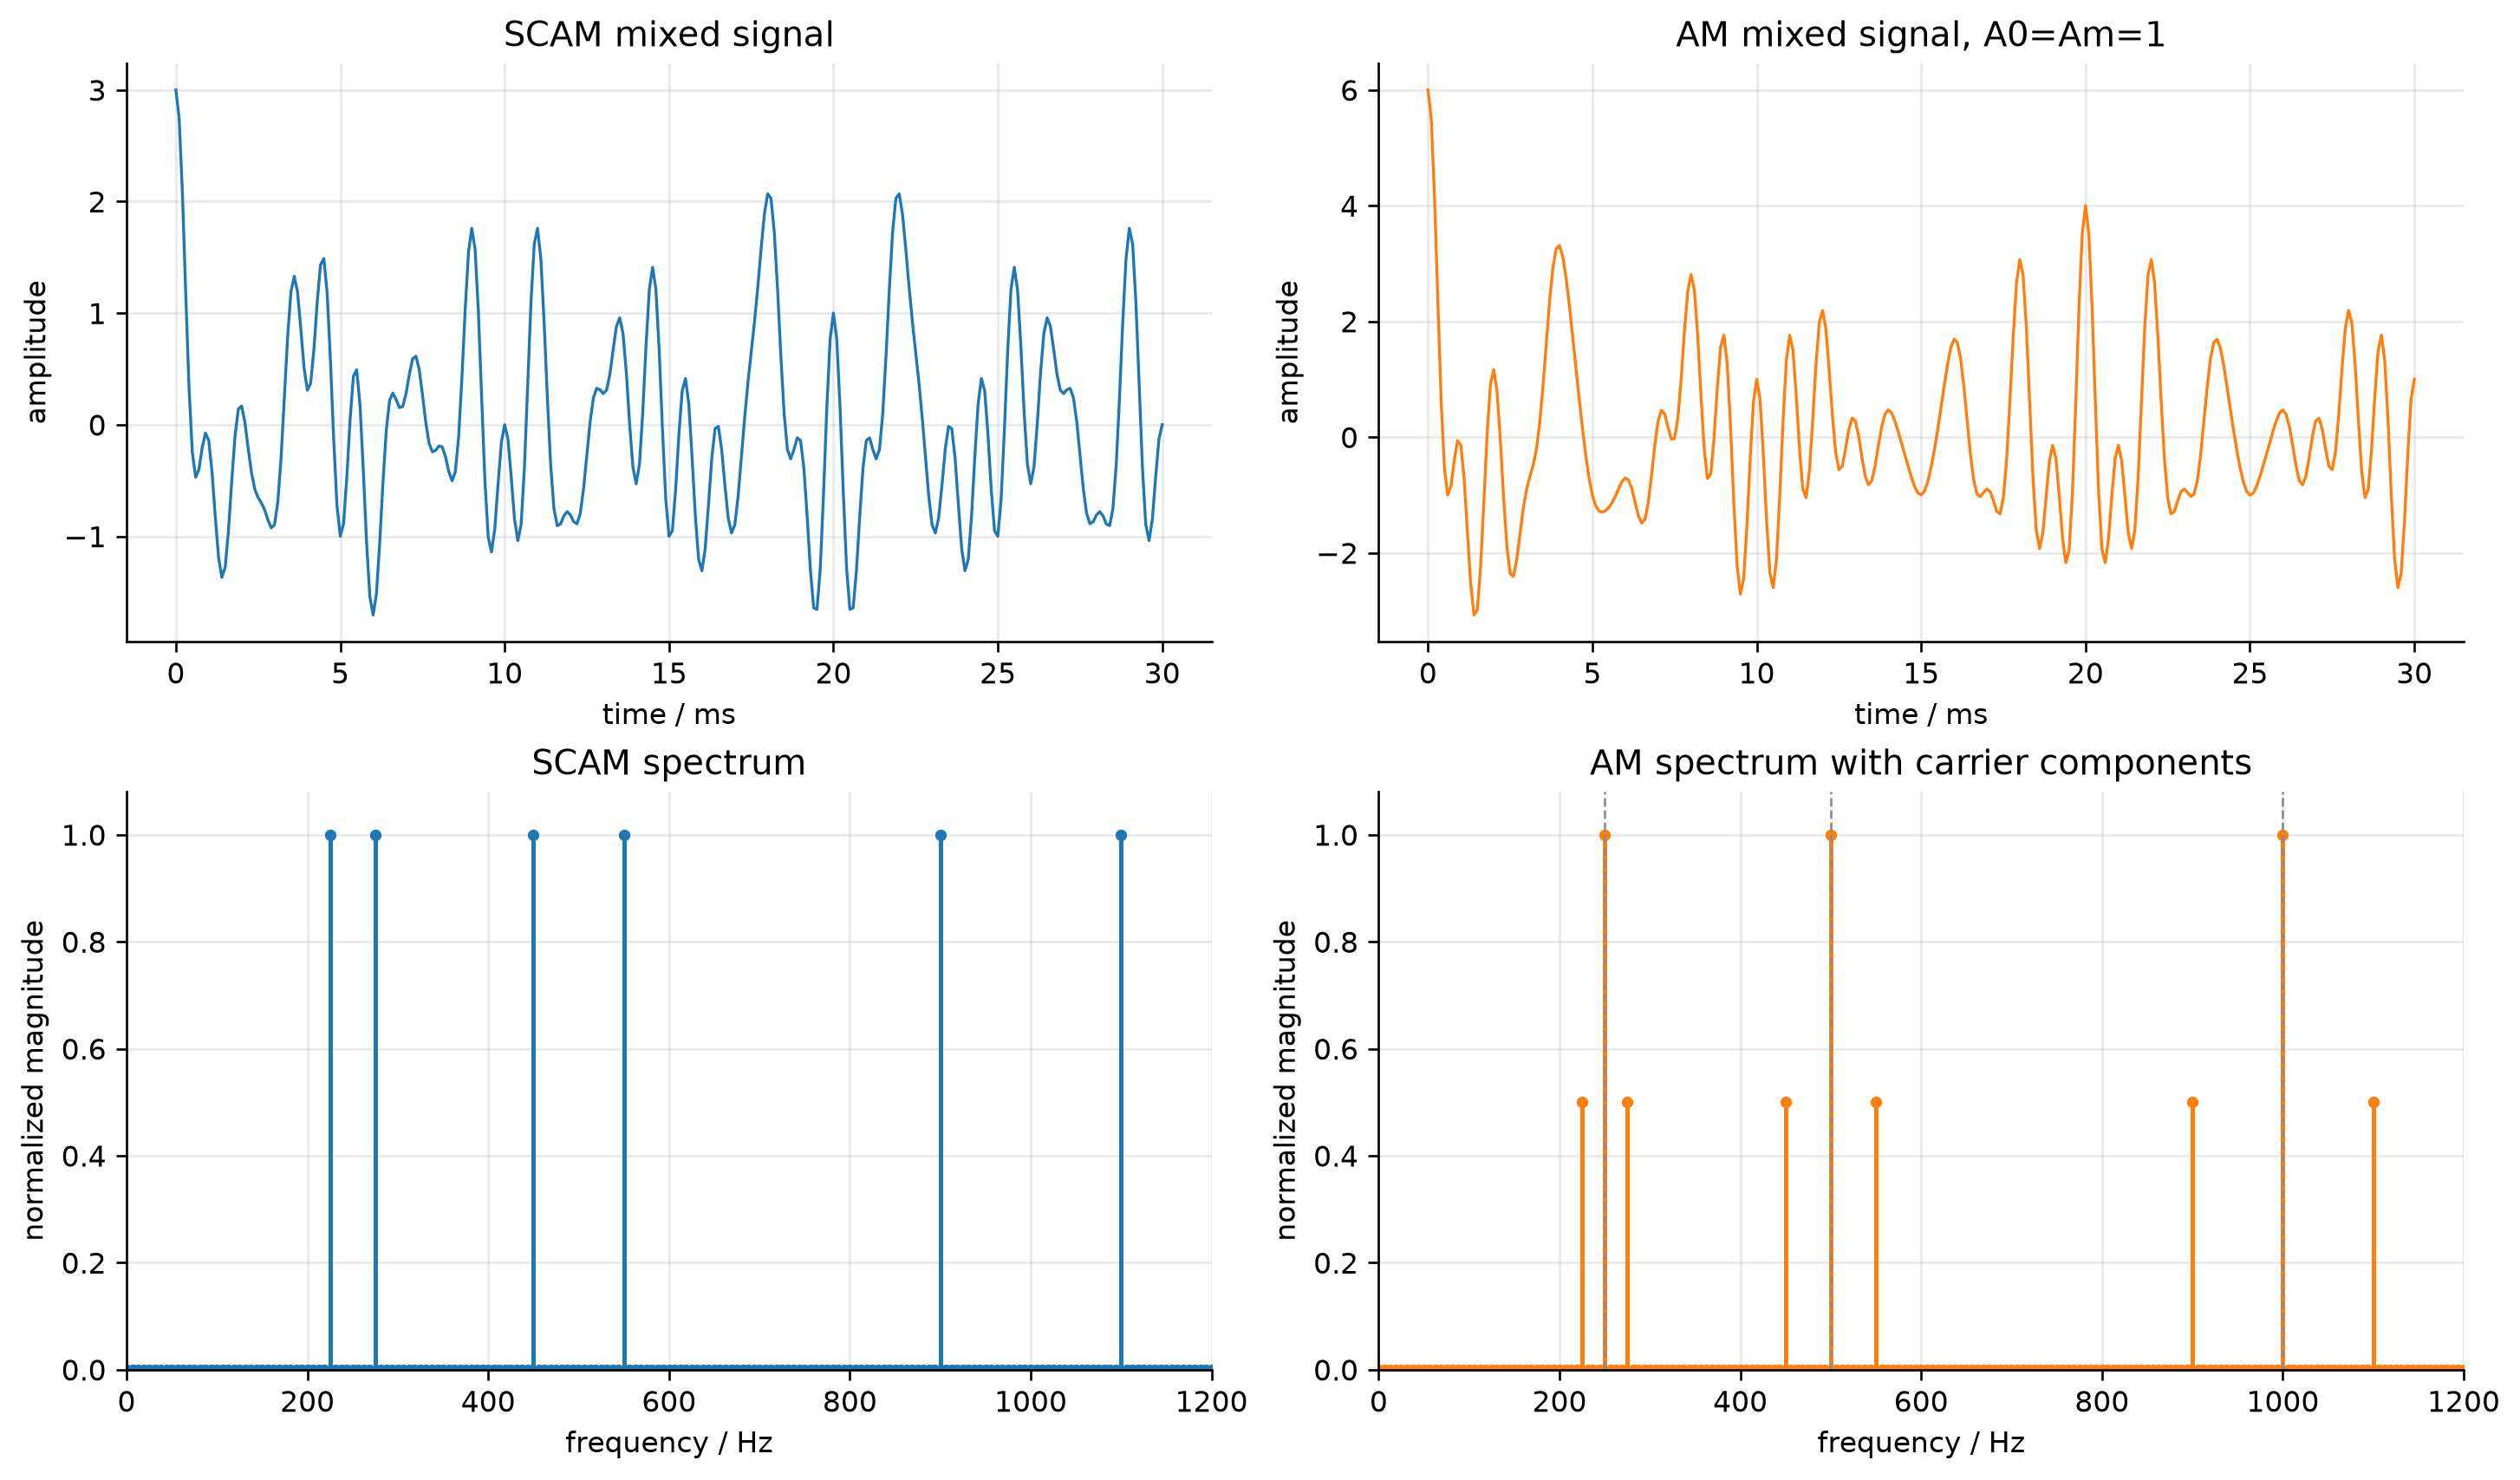
\includegraphics[width=0.95\textwidth]{am_vs_scam.png}
\caption{AM 信号与抑制载波调幅信号的时域和频域对比}
\label{fig:am-scam}
\end{figure}

\appendix
\chapter{程序清单}

\lstset{
  basicstyle=\ttfamily\scriptsize,
  breaklines=true,
  columns=fullflexible,
  frame=single,
  upquote=true,
  showstringspaces=false,
  tabsize=4,
  texcl=false,
  mathescape=false
}
\lstinputlisting[language=Python,caption={实验二 Python 程序},label={lst:program2}]{experiment2.py}

\end{document}
